\section{Data Mining}
Nel Machine Learning, come vedemo prossimamente, non si scrivono istruzioni ma è la macchina che impara direttamente dai dati. Il \textbf{Data Mining} è quella parte dell'informatica che si occupa di cogliere delle relazioni tra grandi quantitativi di dati. L'assunzione che noi facciamo è che il dato dica qualcosa di vero. Ma questa cosa non è sempre vera!

\subsection{Principio di Bonferroni}
Questo principio è esattamente la rappresentazione di ciò che abbiamo appena detto. Esso dice che è possibile imparare un'informazione sbagliata completamente a caso guardando in grandi distribuzioni di dati e trovando uno di quelli che in letteratura vengono chiamati \textit{falsi positivi}.

\subsubsection{Esempio dei malfattori}
Per capire ancora meglio il discorso introdotto, è utile soffermarsi su un esempio discusso a lezione, dove si vuole analizzare la seguente casistica: si vuole prevedere il numero di coppie di malfattori che si trovano negli hotel per organizzare attentati. Questo valore lo troviamo cercando le coppie di persone, su un db di un miliardo di nomi, che si trovano nello stesso hotel almeno 2 volte nell'arco di 3 anni. 
\\
\begin{figure}[th]
    \centering
    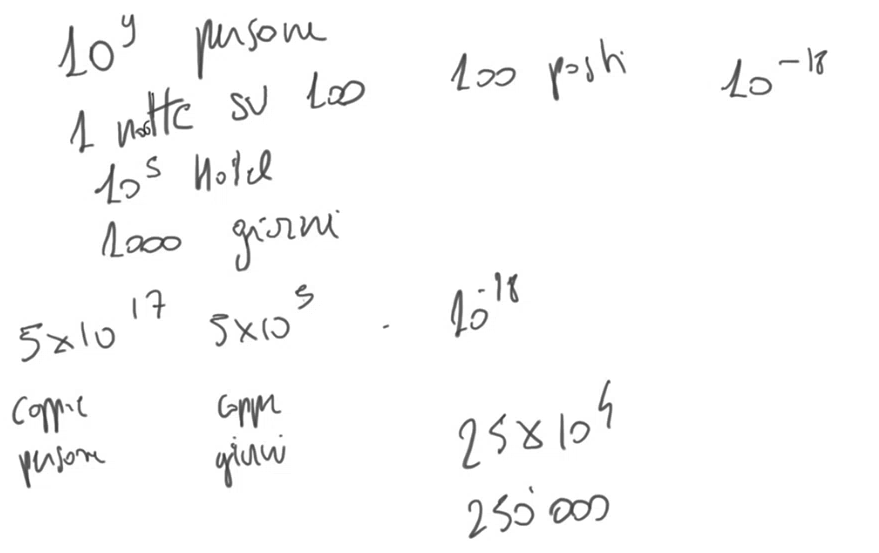
\includegraphics[scale=0.35]{ML/img/Example.png}
    \label{fig:examplex}
\end{figure}
\\
Otteniamo, facendo delle stime di probabilità:
\begin{center}
     $10^{-2}$ probabilità che una persona passi una notte su 100 in hotel
\\[2ex]
    $10^{-2} \times 10^{-2}$ probabilità che due persone passino una notte su 100 in hotel
\\[2ex]
    $\frac{10^{-4}}{10^{5}}$ probabilità che due persone passino una notte nello stesso hotel
\\[2ex]
    $10^{-9} \times 10^{-9}$ probabilità che due persone passino due notti nello stesso hotel nel periodo considerato
\end{center}
E quindi salviamo un $10^{-18}$. Ora calcoliamo: 
\begin{center}
    $\frac{10^9 \times 10^9}{2} = 5 \times 10^17$ numero combinazioni coppie
    $\frac{10^3 \times 10^3}{2} = 5 \times 10^5$ numero combinazioni giorni
\end{center}
E con questi due valori, uniti alla probabilità di trovare una coppia sospetta, calcoliamo il numero atteso di coppie sospette: 
\begin{center}
    $5 \times 10^17 \times 5 \times 10^5 \times 10^{-17} = 250'000$
\end{center}
Ma su un miliardo di persone, è normale trovare anche più coppie che si troveranno nello stesso hotel in quel lasso di tempo, potrebbero essere bambini, persone sposate, persone fidanzate ecc... Quindi è necessario un lavoro sui dati da studiare.

\section{Machine Learning}
\subsection{Perchè utilizzare il Machine Learning?}
Parliamo quindi ora del Machine Learning, e nello specifico, della classica pipeline quando si parla di ML. 
\\
\begin{figure}[th]
    \centering
    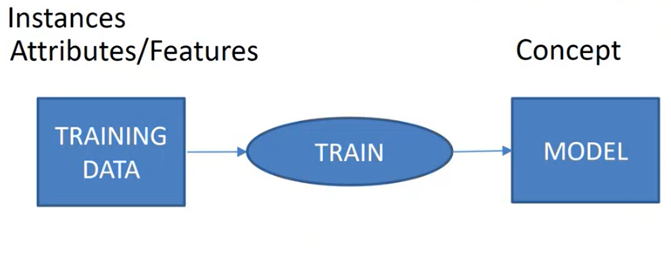
\includegraphics[scale=0.5]{ML/img/MLPipeline.png}
    \label{fig:MLpip}
\end{figure}
\\
Il Machine Learning è la scienza che si occupa di programmare un computer affinchè \textit{impari dai dati}. Gli esempi da cui esso impara vengono chiamati "training instances" e la parte del sistema che impara e fa le prediction è chiamata modello. Neural Networks e Random Forest sono esempi di modelli. 
\\
\textbf{Ma perchè utilizzarlo?} Solitamente, in un qualsiasi codice "automatico" avresti necessità per certi aspetti di elencarglieli uno ad uno: facciamo un esempio più pratico. Scriviamo il codice dello \textit{spam filter} e elenchiamo tutte le possibili parole chiave che ci aiutino a riconoscere gli spam. Se dovessimo sbagliare a scrivere, o queste key dovessero cambiare, saremmo costretti a cambiare il codice. Un modello di ML invece, imparerebbe direttamente dai dati, sopperendo a tutti problemi elencati; potrebbe aggiornarsi per rimanere al passo con gli spam più evoluti e non farebbe errori di trascrizione o riconoscimento. 

\subsection{Tipologie di apprendimento}
Tra le più famose elenchiamo (in ordine sparso):
\begin{itemize}
    \item Classificazione
    \item Regressione
    \item Clustering 
    \item Data Reduction
    \item Association Learning 
    \item Similarity Matching
    \item Profilazione
    \item Link Prediction
    \item Causal Modeling
\end{itemize}


\subsection{Risultato}
Il risultato del ML è un modello che mi genera una predizione con un grado elevato di riuscita. Migliori saranno i dati di input, migliori saranno le predictions. Le istanze di train devono essere ben distribuite e soprattutto devono rappresentare fedelmente la feature su cui si vuole fare una predizione. 
\\
In sostanza, il Machine Learning è utile per:
\begin{itemize}
    \item problemi la cui soluzione richiede molto fine-tuning e un codice spropositato. 
    \item problemi complessi per cui non è possibile utilizzare un approccio tradizionale
    \item enviroments dove i dati sono soggetti a cambiamenti
    \item ottenere informazioni sulle distribuzioni di big data
\end{itemize}

\subsection{Tipologie di modelli}
Un modello di ML quando si distingue per vari criteri:
\begin{itemize}
    \item il tipo di $supervisione$ durante il training
    \item se possono aggiornarsi con il tempo
    \item se lavorano semplicemente sui dati conosciuti, trovando la relazione tra nuovi data e quelli vecchi, o se imparano dei pattern
\end{itemize}
Durante questo corso, abbiamo parlato principalmente di modelli di ML che apprendono in maniera supervisionata, e che non si aggiornano col tempo. 
\\
\textbf{Cosa si intende per studio supervisionato?} Si parla comunemente di $supervised$ ML quando il modello si allena su un training set che contiene già le soluzioni desiderate chiamate $label$. Un esempio sarebbe un dataset dei dati clinici di alcuni pazienti e una feature \texttt{Heart\_Failure} a valori binari [0, 1] che indica se questi pazienti hanno avuto un infarto. Possiamo allenare un modello a prevedere le probabilità di infarto di nuovi pazienti su questo dataset, considerando le cartelle cliniche dei pazienti che l'hanno avuto e la loro sintomatologia. 
\\
Si fa distinzione tra $supervised$ $learning$ e $unsupervised$ $learning$. Nel caso di un apprendimento non supervisionato, come si può dedurre banalmente, il training viene eseguito su un dataset senza una label desiderata: il modello prova ad imparare "senza un istruttore" e quindi le operazioni più frequenti sono quelle di clustering, dove si cerca una relazione di similitudine tra i dati. 
\\
\begin{figure}[th]
    \centering
    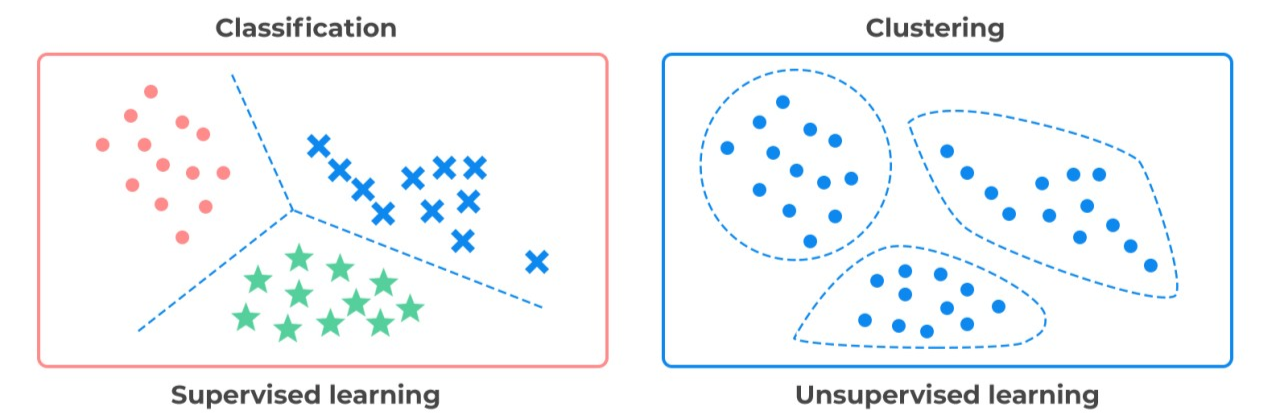
\includegraphics[scale=0.3]{ML/img/sup unsup.png}
    \label{fig:supunsup}
\end{figure}

\newpage

\subsection{Regressione}
\subsubsection{Regressione lineare}
Immaginiamo di voler stimare la qualità della vita di un individuo, a partire dal PIL pro capite. Potremmo quindi indicare la $life\_satisfaction$:
\begin{center}
    $life\_satisfaction$ = $\theta_0$ + $\theta_1$ $\times$ PIL
\end{center}
E avremmo così una relazione lineare tra i due valori (al crescere del PIL, la qualità della vita migliora). Generalmente, un modello lineare fa una prediction calcolando semplicemente una somma pesata delle input features, più una costante chiamata $bias$. 
\begin{itemize}
    \item $\theta_0$ è il bias term, o intercept term
    \item $\theta_1$ è il il peso
    \item PIL (se vogliamo esprimere un generico valore, metteremo $x$) indica la nostra input feature
    \item life\_satisfaction ($y$) sarebbe il valore predetto
\end{itemize}
E ricadiamo nella categoria di \textbf{regressione}.
\\
\textbf{Un modello lineare può essere utilizzato per classificazione?} Certamente. Esistono diversi modelli lineari, che attraverso la separazione dei dati, effettuano classificazione.  
\\
\begin{figure}[th]
    \centering
    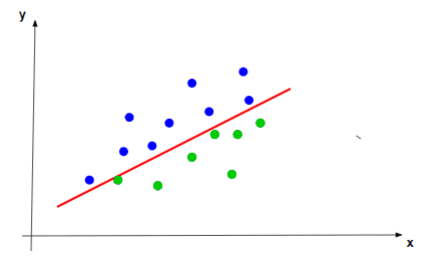
\includegraphics[scale=0.25]{ML/img/class lineare.png}
    \label{fig:linclass}
\end{figure}
\\
Un esempio pratico è il modello SVM, che sfrutta il concetto di $support$ $vector$ per separare linearmente i dati. Entrando nello specifico (ma non troppo) si tratta di $large$ $margin$ $classification$: immagina il classificatore SVM come un modello che cerca di creare la più grande zona di separazione tra le due classi in una distribuzione di dati, usando delle rette parallele. 
\\
\begin{figure}[th]
    \centering
    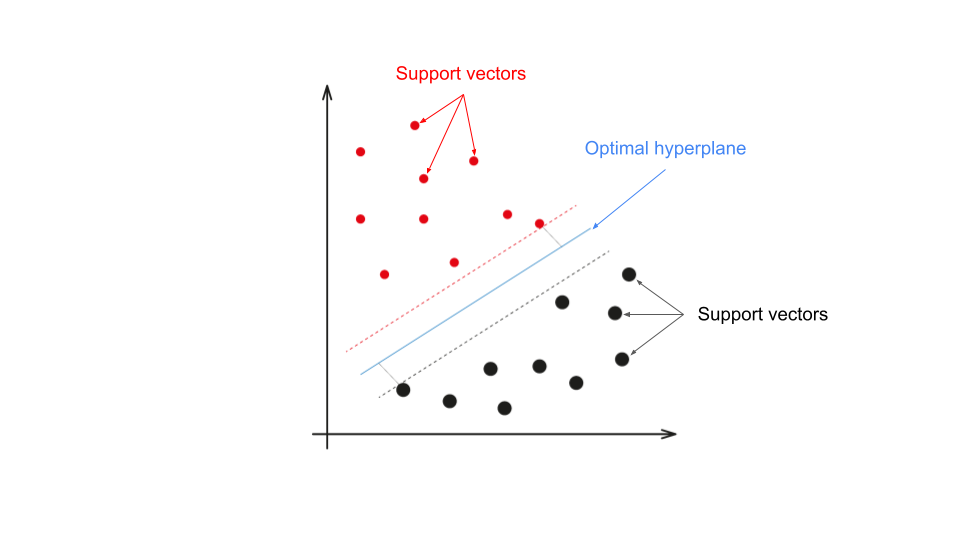
\includegraphics[scale=0.25]{ML/img/hyperplane.png}
\end{figure}
\\
\textbf{Attenzione!} La logistic regression è un classificatore binario che non fa rette, ma semplicemente calcola la probabilità che una classe sia 1 rispetto alla probabilità che sia 0 ed è quindi diverso dalla linear regression. (\textit{Il prof bene o male ha detto solo questo sulla logistic regression.})

\newpage

\subsubsection{Decision Tree}
Uno dei modelli più versatili in ML, il Decision Tree (o albero decisionale) può essere utilizzato per classificazione e regressione, ma anche in casi con multiple outputs. Sono algoritmi molto potenti che possono essere sfruttati per dataset complessi. 
\\
\begin{figure}[th]
    \centering
    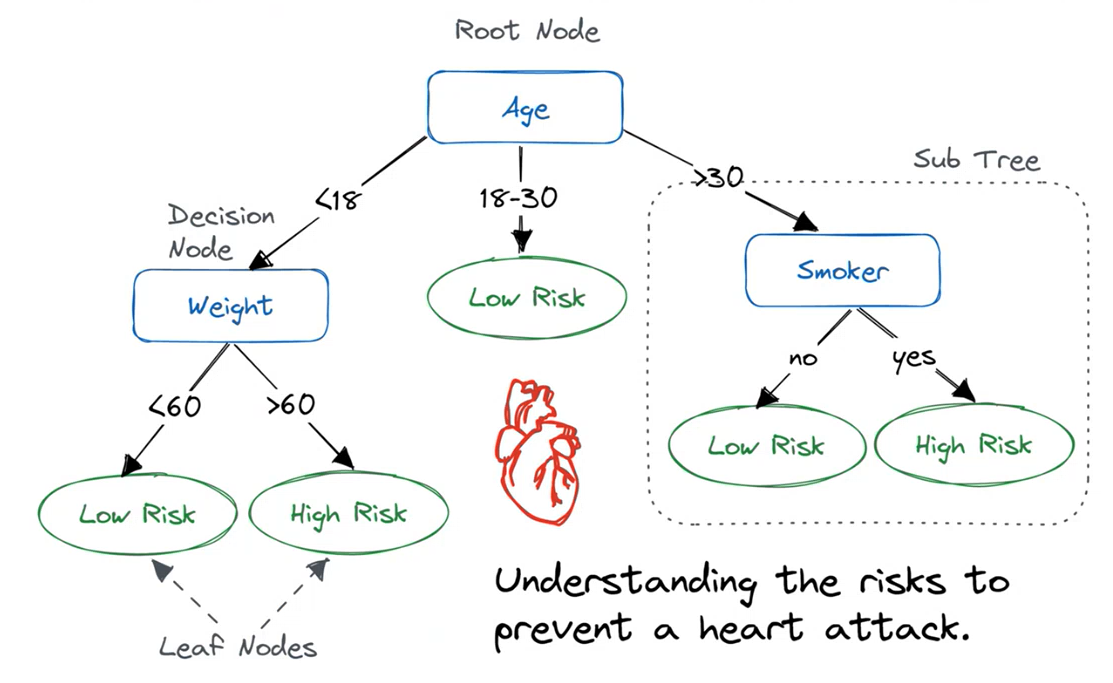
\includegraphics[scale=0.5]{ML/img/decision tree.png}
\end{figure}
\\
Uno dei suoi punti di forza è la sua leggibilità: un altro aspetto molto ricercato nei modelli di ML è la facilità di comprensione del modello.
\\
Il Binary Decision Tree è sicuramente uno dei più semplici da leggere e viene detto $white$ $box$ $model$, ovvero modello a "scatola bianca", indicando l'opposto di una scatola nera. La problematica dell'interpretabilità nel ML è ancora oggi affrontata e ha l'obiettivo di capire sempre meglio il tipo di ragionamento fatto dai modelli e tradurlo in qualcosa che l'umano possa capire; si ha questa necessità per influenzare sempre meglio le scelte che vengono fatte dagli algoritmi, soprattutto influenzarli per una questione di $fairness$.
\\
Nel Decision Tree si ha un Root node iniziale, da cui partono i primi rami, che arrivano a degli altri nodes (se a loro volta hanno delle diramazioni) o a delle leaves (o foglie, se sono nodi terminali). E sicuramente un altro pro dei Decision Trees è che non richiedono una grossa $data$ $preparation$.
\\
\textbf{Esempio di lettura.} Partendo dall'immagine qui sopra, cerchiamo di capire il ragionamento di un modello ad alberi decisionali. Si vuole prevedere il rischio di un paziente di avere un infarto (Sì lo so siamo tornati su questo brutto esempio). 
\\
L'albero parte da una feature, \texttt{Age}:
\begin{center}
    \textit{In quale gap di età si trova il paziente?}
\end{center}
E genera tre leaf nodes: $<$18, 18-30, $>$30.
\\
Poi scopre dal dataset che la maggior parte delle persone con età compresa tra 18 e 30 anni, sono a basso rischio, a prescindere da altri fattori (che in letteratura vengono chiamati feature). 
\\ 
Analizzando in età minore di 18, nota che c'è una feature che fa pendere l'ago della bilancia: \texttt{Weight} (peso): crea quindi due leaf nodes con rischio alto e basso sulla base di tale valore. 
\\
Discorso analogo si fa per le persone con più di 30 anni dove però la feature critica è \texttt{Smoker}.
\\[3ex]
\textbf{N.B. Decision Tree può essere anche letto come un insieme di regole, ognuna che ci porta una risposta.}

\newpage

\subsubsection{Costruzione di un Decision Tree}
Per costruire un Decision Tree, scegliamo il primo nodo e dividiamo le istanze di quell'attributo. Come si sceglie l'attributo di partenza?
\\
\begin{figure}[th]
    \centering
    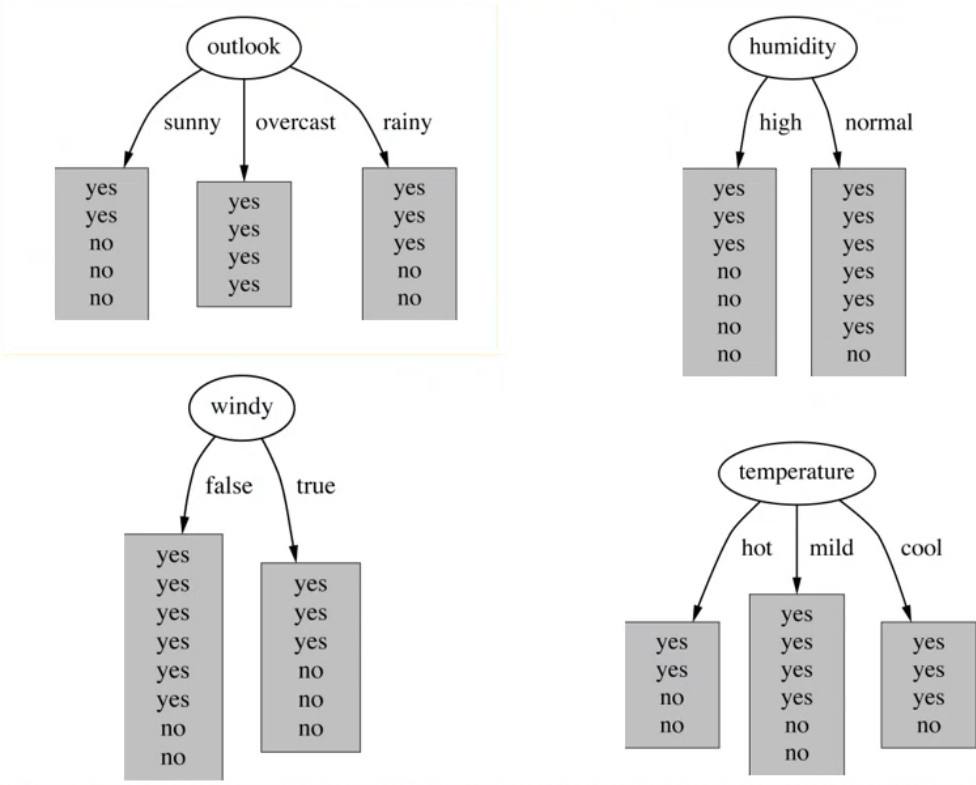
\includegraphics[scale=0.5]{ML/img/dt_scelta.png}
\end{figure}
\\
Tra questi attributi, la scelta ottimale è Outlook. Questo perchè è l'unico a darci l'informazione migliore su una delle sue istanze: overcast. Overcast ha una probabilità del 100\%. Ogni volta che c'è tempo nuvoloso, si gioca a calcetto. Non è necessario pruning o altre operazioni sull'albero, quella è già una foglia, a differenza degli altri che si dirameranno. Ma quando creo un albero decisionale devo formarlo il più efficiente possibile: ogni nodo deve massimizzare l'information gain. 
\\
Questo ragionamento, viene trodotto in linguaggio matematico nel calcolo dell'entropia per ogni attributo:
\begin{itemize}
    \item Entropia del nodo Outlook, data dalla somma tra le entropie (Sunny, Overcast, Rainy):
    \begin{center}
        \begin{math}
            info_{Sunny} = entropy(2/5, 3/5) = -\frac{2}{5} log(\frac{2}{5}) - \frac{3}{5} log(\frac{3}{5}) = 0,971 bits  
        \end{math}
        \\[2ex]
        \begin{math}
            info_{Overcast} = entropy(4,0) = -\frac{4}{4} log(\frac{4}{4}) - \frac{0}{4} log(\frac{0}{4}) = 0  
        \end{math}
        \\[2ex]
        \begin{math}
            info_{Rainy} = entropy(3/5, 2/5) = -\frac{3}{5} log(\frac{3}{5}) - \frac{2}{5} log(\frac{2}{5}) = 0,971 bits
        \end{math}   
        \\
    \end{center}
    \item L'informazione attesa è:
    \begin{center}
        \begin{math}
            info[(2,3), (4,0), (3,2)] = (\frac{5}{14}) \times 0,971 + (\frac{4}{14}) \times 0 + (\frac{5}{14}) \times 0,971 = 0,693 bits
        \end{math}
    \end{center}
    \item Mentre l'info gain effettiva di Outlook è:
    \begin{center}
        \begin{math}
            gain(Outlook) = info([9,5]) - info([2,3], [4,0], [2,3]) = 0,247 bits
        \end{math}
    \end{center}
\end{itemize}
Il risultato è che facendolo con anche gli altri, il valore con info gain più elevato è proprio Outlook. Per costruire l'albero, itero questo procedimento negli attributi sotto. 

\newpage

\subsubsection{Simple Algorithm}
Come trasformo il Decision Tree in una regola? Esiste una procedura iterativa, dove cerchiamo di massimizzare l'accuracy della stessa.Tenendo in considerazione il numero di istanze a cui si applica la regola e al numero di quelli a cui si applica correttamente e massimizzando il loro rapporto.
\\
\textbf{Esempio.} Immaginiamo di avere un dataset con i dati sulla vista di alcune persone. La regola? Vogliamo capire qual è il tipo corretto di lenti per una persona non vedente. Sappiamo diverse sue caratteristiche fisiche. Potenzialmente, una regola potrebbe essere "Altezza $>$ 1.80". Andiamo a contare nel dataset per quante persone servono le lenti ,che sono sopra a l'1.80, e si fa il rapporto tra casi positivi / casi considerati dalla regola. Potremmo avere 4 persone con necessità su 45 considerate. La regola sarebbe molto debole. 
\\
\begin{figure}[th]
    \centering
    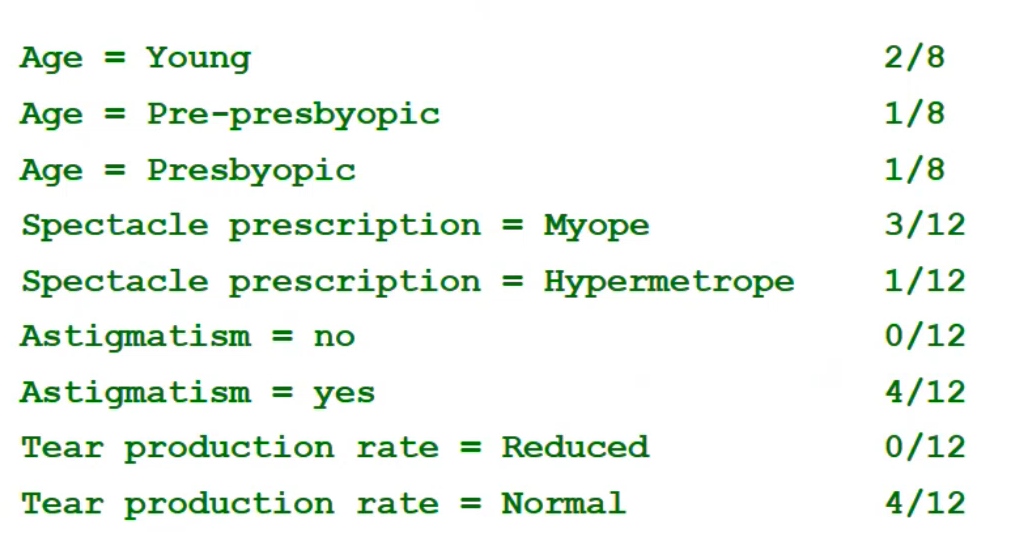
\includegraphics[scale=0.35]{ML/img/dataset_lenses.png}
\end{figure}
\\
Cosa prendiamo? La regola che massimizza il rapporto. Quindi prenderemo Tear production rate = normal oppure astigmatism = yes, e ne scegliamo una delle due (hanno lo stesso valore). Andiamo avanti come nel Decision Tree con le altre righe del dataset e le nuove regole e le combino tutte. Però non devo renderlo troppo specifico, altrimenti non generalizza!

\subsection{Overfitting}
Uno dei problemi più importanti dell'intero ML e consiste in un modello che performa bene sui dati di training, ma non è capace di generalizzare, sbagliando completamente nel test. Questo succede per dataset troppo specifici, o per noise all'interno di essi che il modello interpreta come pattern e impara. Il modello in sè non è capace di distinguere questi noises. 
\\
\textbf{Esempio.} Immaginiamo di allenare un modello a prevedere da un dataset, l'altezza di un cittadino cinese dalle sue caratteristiche. Il test però lo eseguiamo su un dataset di persone provenienti dalla Svezia. Sicuramente, l'accuracy sarà bassissima, ma questo è dovuto non al modello scelto, ma alla scelta del dataset su cui efftuare train e test.
\\
\textbf{Quindi come lo evito?} Basta $discretizzare$ l'intervallo delle temperature in insiemi, generalizzando.

\subsubsection{i.i.d. assumption per Statistical Modeling}
Abbiamo due particolari assunzioni da fare nel caso dello statistical modeling:
\begin{itemize}
    \item tutti gli attributi sono ugualmente importanti (identically distributed)
    \item tutti gli attributi sono statisticamente indipendenti (independent distributed)
\end{itemize}
Ma sappiamo che la seconda è impossibile da garantire, basta guardare il dataset metereologico e pensare che gli attributi di tempo e umidità sono dipendenti.

\newpage

\subsection{Instance based learning}
Viene descritta come la più semplice forma di apprendimento: non si impara nulla, si fa tutto a memoria, con una funzione di istanza (quanto l'elemento A è simile a B o C ecc..) un esempio sono gli algoritmi simili al nearest neighbours. 
\\ 
Sono una serie di modelli molto utilizzati per fare profilazione e cercare le preferenze di un utente. La tipologia più conosciuta di instance learning è il nearest neighbors, un modello dove cerco "tutte le istanze più vicine". Ci sono alcuni accorgimenti da fare per poterlo utilizzare, uno di essi è la necessità di normalizzare il dataset altrimenti overfitta. 

\subsection{One rule algorithm}
Inventato nel '94, è l'algoritmo più banale di tutti. Da un dataset, estrae una sola regola. L'idea alla base è molto semplice, tuttavia non è da sottovalutare: spesso le idee semplici sono quelle più efficaci.
\\
\begin{figure}[th]
    \centering
    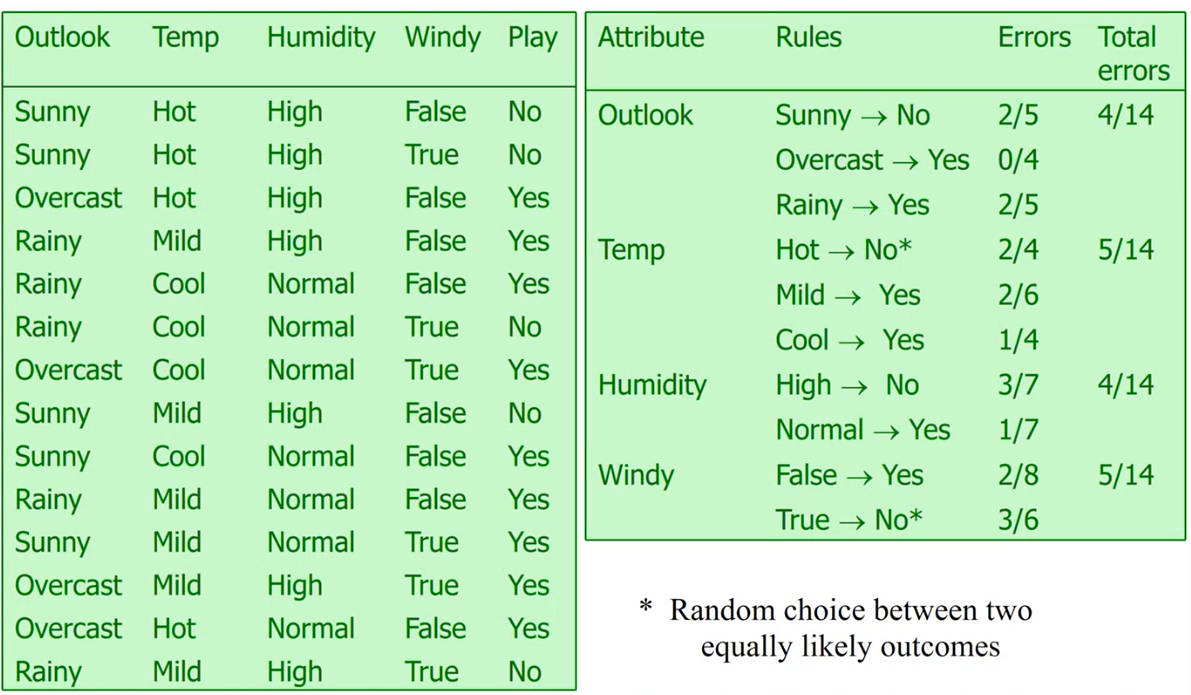
\includegraphics[scale=0.5]{ML/img/onerule.png}
\end{figure}
\\
Analizziamo questo dataset e il potenziale risultato del one rule. Immaginiamo di dover prevedere se giocare a calcetto, sulla base del meteo; contiamo per ogni l'attributo \texttt{Outlook} i valori distinti di play. Ad esempio, per \texttt{Outlook} = \texttt{Sunny} notiamo che è \texttt{No} 3 volte su 5, il che significa che commette 2 errori su 5. E li contiamo per ogni valore di ogni feature. Alla fine prendiamo come rule la feature su cui commettiamo meno errori totali: in questo esempio, una a scelta tra \texttt{Humidity} e \texttt{Outlook}.
\\
\textbf{Quale errore commette il one rule?} Il motivo per cui è poco utilizzato, risiede proprio nella sua semplicità. Seguendo il suo modus operandi, è utile notare che: per valori numerici ad intervalli grandi, diventa impossibile contare gli errori. Ad esempio, se aggiungessimo l'attributo temperatura, con tanti valori di temperature in un intervallo compreso tra i 15 e i 25 gradi, lui imparerebbe una rappresentazione troppo dettagliata, causando $overfitting$.

\newpage

\subsection{Naive Bayes Classifier}
Come funziona un classificatore probabilistico? Calcola la probabilità che un evento si verifichi, basandosi sulla distribuzione di probabilità del dataset di training. 
\\
\begin{figure}[th]
    \centering
    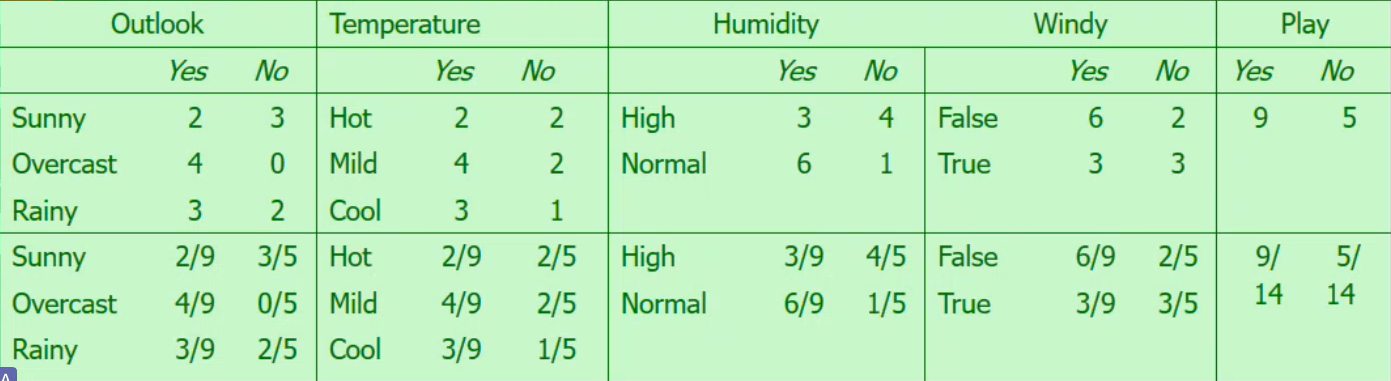
\includegraphics[scale=0.5]{ML/img/prob class.png}
\end{figure}
\\
Tornando alla tabella del calcetto, calcolo la probabilità di fare un calcetto per ogni valore di ogni attributo. 
\\
\begin{figure}[th]
    \centering
    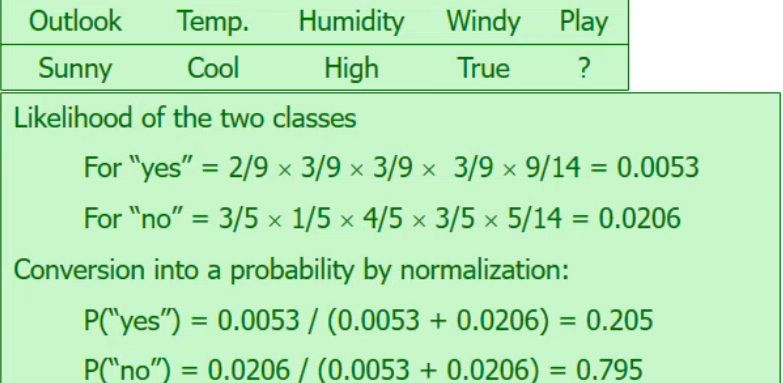
\includegraphics[scale=0.5]{ML/img/new day.png}
\end{figure}
\\
Osservando il nuovo giorno e sulla base dei dati di training è possibile calcolare la probabilità che si faccia il calcetto o no. Utilizzo la probabilità che sia sì, e quella che sia no, e ricavo la likelihood facendo:
\begin{center}
    \begin{math}
        p_{newday}(Yes) = \frac{p(Sunny)}{p(Yes)} + \frac{p(Cool)}{p(Yes)} + \frac{p(High)}{p(Yes)} + \frac{p(True)}{p(Yes)}
    \end{math}
    \\
    \begin{math}
        p_{newday}(No) = \frac{p(Sunny)}{p(No)} + \frac{p(Cool)}{p(No)} + \frac{p(High)}{p(No)} + \frac{p(True)}{p(No)} 
    \end{math}
\end{center}
Le normalizzo a uno:
\begin{center}
    $p(Yes)$ = $\frac{p_{newday}(Yes)}{p_{newday}(Yes) + p_{newday}(No)}$
    \\
    $p(No)$ = $\frac{p_{newday}(No)}{p_{newday}(Yes) + p_{newday}(No)}$
\end{center}
E ottengo lo score delle due risposte. Eseguo quindi una classificazione probabilistica.

\newpage

\subsubsection{Regola di Bayes}
\begin{center}
    \begin{math}
        Pr[ H | E] = \frac{Pr[E | H] Pr[H]}{Pr[E]}
    \end{math}
\end{center}
Questa regola viene descritta nel modo seguente:
\begin{center}
    \textit{La probabilità di un evento H, data un evidenza E, è uguale alla probabilità dell'evidenza dato un evento, moltiplicata per la probabilità dell'evento e diviso la probabilità dell'evidenza.}
\end{center}
Che spiegato in termini semplici, ritornando quindi all'esempio del calcetto:
\begin{itemize}
    \item L'evidenza sarebbe la nuova riga di ds da classificare.
    \item L'evento sarebbe: si gioca o non si gioca?
    \item Quindi, il primo termine nella frazione sarebbe la probabilità che ci siano certe condizioni quando si verifica l'evento: se la nuova riga da classificare dice che c'è soleggiato, umido, una certa temperatura... quel termine indica la probabilità che se si gioca a calcetto, ci siano esattamente quelle condizioni, che è diverso dal chiedersi se con quelle condizioni si gioca a calcetto.
    \item Questo termine è poi moltiplicato per la probabilità che si giochi (ricavabile dai dati di training)
    \item Il termine al denominatore è l'unica incognita in questa formula. Consiste nella probabilità a priori dell'evidenza. Ovvero, la probabilità che si verifichi una certa giornata nel nostro caso (ovvero che ci sia una giornata soleggiata, con una certa temperatura ecc...). Valore non calcolabile perchè ci servirebbero tutti i valori delle giornate del mondo!
    \item La soluzione a questo problema consiste nell'evitare il denominatore. Alla fine, è un valore per cui vengono divise entrambe le probabilità: sia che l'evento H si verifichi, sia che non si verifichi, il valore al numeratore cambia ma il denominatore no: lo consideriamo un valore inutile e non lo ricaviamo.
\end{itemize}
Il classificatore Bayesiano sfrutta questo concetto. Il Naive Bayes invece va oltre: 
\\
\begin{itemize}
    \item Andando a pescare tra le i.i.d. assumption, considera le feature indipendenti tra loro, quindi il primo termine al numeratore, lo scompone nella produttoria tra tutte le probabilità delle evidenze dato H. Considerando le feature indipendenti, consideriamo la probabilità dell'evidenza E dato l'evento H come l'unione delle probabilità di eventi indipendenti, ovvero la produttoria dei singoli elementi disgiunti. Il numeratore diventa quindi
    \begin{center}
        \begin{math}
            Pr[ H | E] = \frac{Pr[E_1 | H] Pr[E_2 | H] Pr[E_3 | H] ... Pr[E_n | H] Pr[H]}{Pr[E]}
        \end{math}
    \end{center}
\end{itemize}
\textbf{Qual è il problema di questo approccio?} Che se la probabilità di un'evidenza dato l'evento è 0, mi porta tutto a 0. 
\\
\textbf{Come posso evitare questo problema?} Aggiungo 1 al conteggio per ogni combinazione valore attributo-classe. 

\newpage    

\subsection{Unsupervised Learning}
\subsubsection{Clustering}
Si parla di learning unsupervised quando non si utilizzano label. Quindi non è nota la classe da predire. Quello che avviene nel clustering quindi è una divisione naturale delle istanze in gruppi. 
\\
Come funziona l'algoritmo gerarchico? Finchè non ci fermiamo, cerchiamo i migliori due cluster da unire e li uniamo. Altrimenti esiste anche probabilistico: basta trovare la probabilità che un certo punto appartenga al cluster i-esimo. Come si trova la distanza tra due cluster? Sfrutti i loro centroidi (sono punti medi) e cerchi quelli più vicini. Possiamo capire quanti cluster creare, basta organizzare un dendrogramma e separarlo dove avviene la separazione principale. 
\\
\begin{figure}[th]
    \centering
    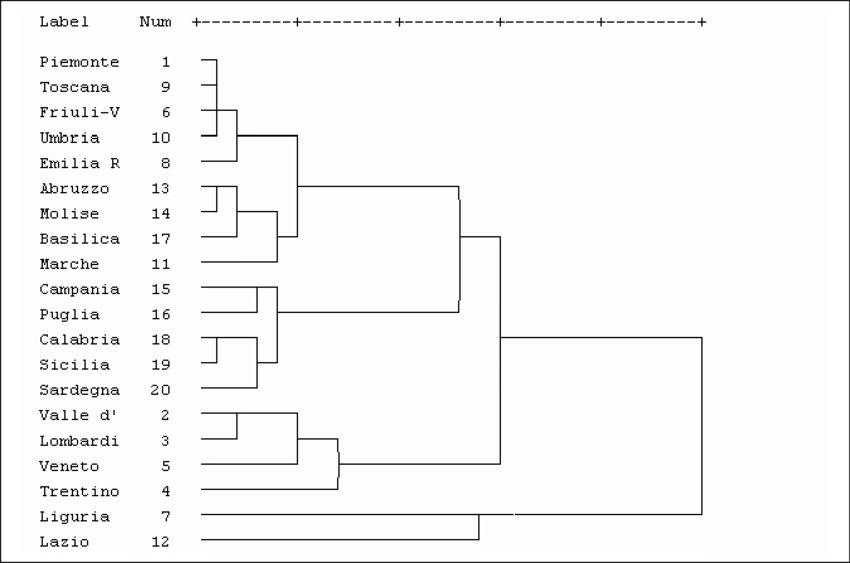
\includegraphics[scale=0.5]{ML/img/dendrogramma.png}
\end{figure}

\newpage

\subsection{Come trovo un modello che non overfitta?}
Per calcolare l'overfitting del modello, separiamo il dataset in due parti, training e test. 
\\
Per vedere una misura dell'overfitting, basta guardare la misura dell'errore, sia nella simulazione reale che durante la fase di training. Per capire effettivamente quando un modello overfitta, è necessario guardare la sua complessità: più un modello è complesso, più \textit{tenderà ad overfittare.}
\\
Il Decision tree è un modello che tende ad overfittare: se immaginiamo un albero molto dettagliato, con tanti rami e nodi che descrivano ogni possibile feature del dataset, allora overfitteremo sul training set.

\subsection{Come posso aiutare il modello contro l'overfitting?}
Si può suddividere il dataset in tre parti: train, validation, e test set. Il validation è utilizzato per un test prima del test, poi lo traino nuovamente su anche quello. In questo modo separo correttamente training e testing ma soprattutto posso usare i validation data per aggiornare i parametri di learning. 
\\
Esiste un altro metodo chiamato comunemente \textbf{Cross Validation}. Che spiegato molto brevemente, consiste nella suddivisione del dataset in k subsets grandi uguali. A turno, uno solo viene usato per il testing, gli altri per il training. Anche questa tipologia di struttura per la suddivisione del dataset viene utilizzata per fare il tuning dei parametri del modello.

\subsection{Valutazione del modello}
Come si misura l'errore in un modello di ML? Si usa una matrice chiamata \textit{Confusion Matrix} o matrice di confusione; essa mette a confronto le predizioni corrette e quelle sbagliate, toccando il tema dei falsi positivi e falsi negativi, distinguendo tra i due tipi di errore. 
\\
\begin{figure}[th]
    \centering
    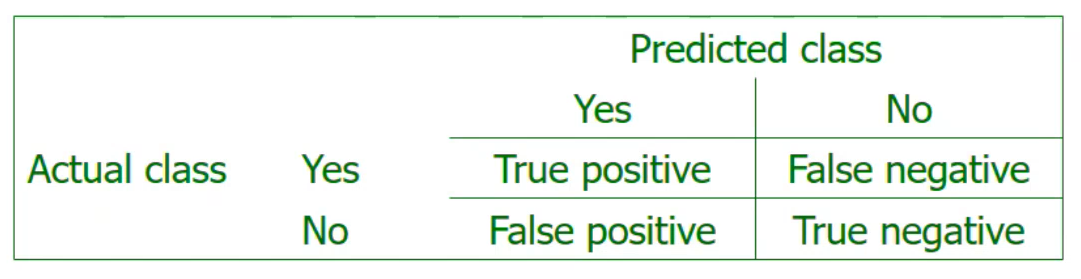
\includegraphics[scale=0.5]{ML/img/conf_matrix.png}
\end{figure}
\\
Sulla base di questa tabella, possiamo definire due parametri:
\begin{center}
    $TP_{rate}$ = $\frac{TP}{TP + FN}$
    \\[2ex]
    $FN_{rate}$ = $\frac{FN}{TN + FP}$
\end{center}
Che rappresentano i rate dei veri positivi e dei falsi negativi. Quindi sarebbero l'accuracy sul Sì, e l'altro è 1 - l'accuracy sulla predizione di No.
\\
Attenzione! Un errore di falso positivo e di falso negativo hanno pesi diversi, e dipendono molto dall'ambiente in cui ci troviamo. 
\\ 
Altre misure che posso ricavare dalla confusion matrix sono la \textit{precision} e la \textit{recall}:
\begin{center}
    $precision$ = $\frac{TP}{TP + FP}$
    \\[2ex]
    $recall$ = $\frac{TP}{TP + FN}$
\end{center}
La precision è un valutare quante di quelle che sono positive, lo sono effettivamente. Non è sufficiente, serve anche la recall che misura quali sono quelli effettivamente scoperti come positivi?

\newpage

\subsubsection{F1 score}
Le due misure indicate nel punto precedente possono essere combinate in una unica: 
\begin{center}
   $F1_{score}$ = $\frac{(\beta^2 + 1) PR}{\beta ^2 P + R}$
\end{center}
Dove il parametro $\beta$ funge da ago della bilancia: quando è $<$ 1, prevale la precision, quando è maggiore la recall e se è uguale vengono considerate in egual modo. 

\subsubsection{Multilabel Confusion Matrix}
Quello visto finora è il caso di classificazione binaria, un conto dei Sì e No. Ma se la label da predire fosse a più valori, quindi non ci trovassimo più in un caso binario, il tipo di matrice sarebbe il seguente:
\\
\begin{figure}[th]
    \centering
    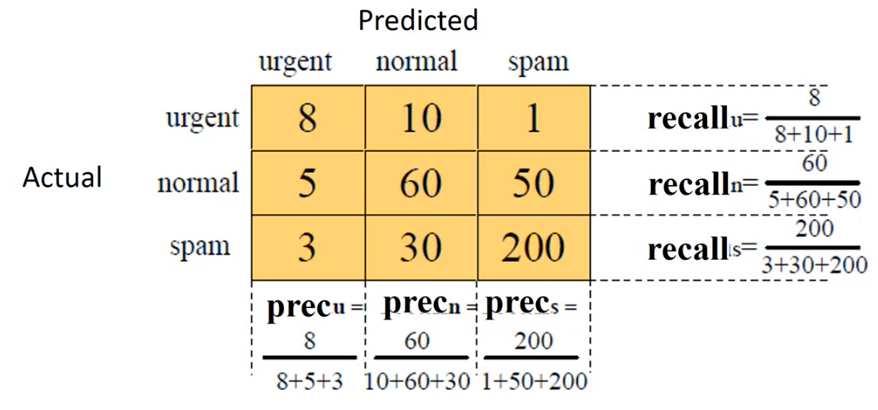
\includegraphics[scale=0.55]{ML/img/multilabel matrix.png}
\end{figure}
\\
Dove precision e recall sono calcolati singolarmente per ogni valore. Questo sistema può essere utilizzato per valutare la logistic regression. 

\subsection{Ensemble learning}
Normalmente i modelli visti si combinano. Ed esistono 2 modi per metterli insieme.
\subsubsection{Bagging}
Separo il dataset in \textit{bags.} Immaginiamo di avere n bags, utilizziamo n modelli e li applico in parallelo su una sola frazione del dataset. 
\subsubsection{Boosting} 
Se il bagging era in parallelo, questo consiste nel mettere in serie i modelli, e quindi tutti i dati passano all'interno di un modello dopo l'altro.